\section{Benchmarks}
\label{sec:bench}

This section compares the performance of our implementations in two dimensions.
First, we compare the successive algorithmic refinements using the \haskell
implementation presented in \cref{sec:motivation} and \cref{sec:improvements}.
Second, we compare different choices of data structures to represent segments
using the \ocaml implementation described in \cref{sec:ocaml}.

All benchmarks were done on a ThinkPad T470 with an i5-7200U CPU and 12G of memory.
The \haskell benchmarks use the Stackage LTS 10.8 release and the \texttt{-O2} option.
The OCaml benchmarks use \ocaml 4.06.1 with the flambda optimizer and the
\texttt{-O3} option. We annotate functors
with the \code{[@inline]} annotation to ensure that functors are applied at
compile time and their content benefits from available optimizations.

\subsection{Comparing Algorithms in the \haskell Implementation}

\cref{sec:motivation} and \cref{sec:improvements} develop the
algorithm for generating languages in a sequence of changes applied to
a naive baseline algorithm. We now evaluate the impact of these
changes on performance, which we plan to measure in terms of
generation speed in words per second. It turns out that this speed
depends heavily on the characteristics of the the regular expression
considered. For that reason, we choose three representative regular expressions to highlight the
strengths and weaknesses of the different approaches.
\begin{itemize}
\item $\Rstar a$: This expression describes a very small language with $P (w\in L) = 0$.
  Nevertheless, it puts a lot of stress on the underlying
  append operation on words as their length increases very quickly.
  The input language contains only one segment whereas all segments of
  the output language contain exactly one element. This combination
  highlights the usefulness of sparse indexing and maps.
\item $\Rstar{(\Rconcat{a}{\Rstar{b}})}$: On the opposite end of the
  spectrum, the language of this regular expression is fairly large
  with $P (w\in L)=0.5$. The expression applies \code{star} to a
  language where segment $n+1$ consists of the word $ab^n$. Its
  evaluation measures the performance of \code{star} on a non-sparse
  language and of {concatenation} applied to a finite and an infinite
  language.
\item $\Rconcat{\Rcomplement{(\Rstar{a})}}{b}$: Finally, this regular
  expression exercises the complement operation and tests the
  concatenation of a very large language, 
  $P (w\in \Lang{\Rcomplement{(\Rstar a)}}) = 1$, to a much smaller
  language.
\end{itemize}

In the evaluation, we consider five variants of the Haskell implementation.
\begin{itemize}
\item The \textbf{naive} implementation corresponds to the code developed by
  the end of Section~\ref{sec:motivation}. It transforms to and from
  segments on the fly and it uses plain list indexing in the
  implementation of concatenation and closure.
\item The \textbf{seg} implementation uses the infinite list-based segmented
  representation throughout (Section~\ref{sec:segm-repr}). Moreover,
  it relies on using maps and sparse indexing
  (Sections~\ref{sec:map-data-structure} and~\ref{sec:sparse-indexing})
  for concatenation and closure.
\item The \textbf{segConv} implementation uses finite and infinite
  segment lists, but it applies the convolution approach
  (Section~\ref{sec:convolution}) to implement concatenation and
  closure.
\item The \textbf{ref} implementation uses the specialized segmented
  representation from Section~\ref{sec:more-finite-repr} combined with
  maps and sparse indexing.
\item The \textbf{refConv} implementation uses the specialized
  segmented representation from Section~\ref{sec:more-finite-repr}
  combined with convolution.
\end{itemize}

\begin{figure}[!tp]
  \centering
  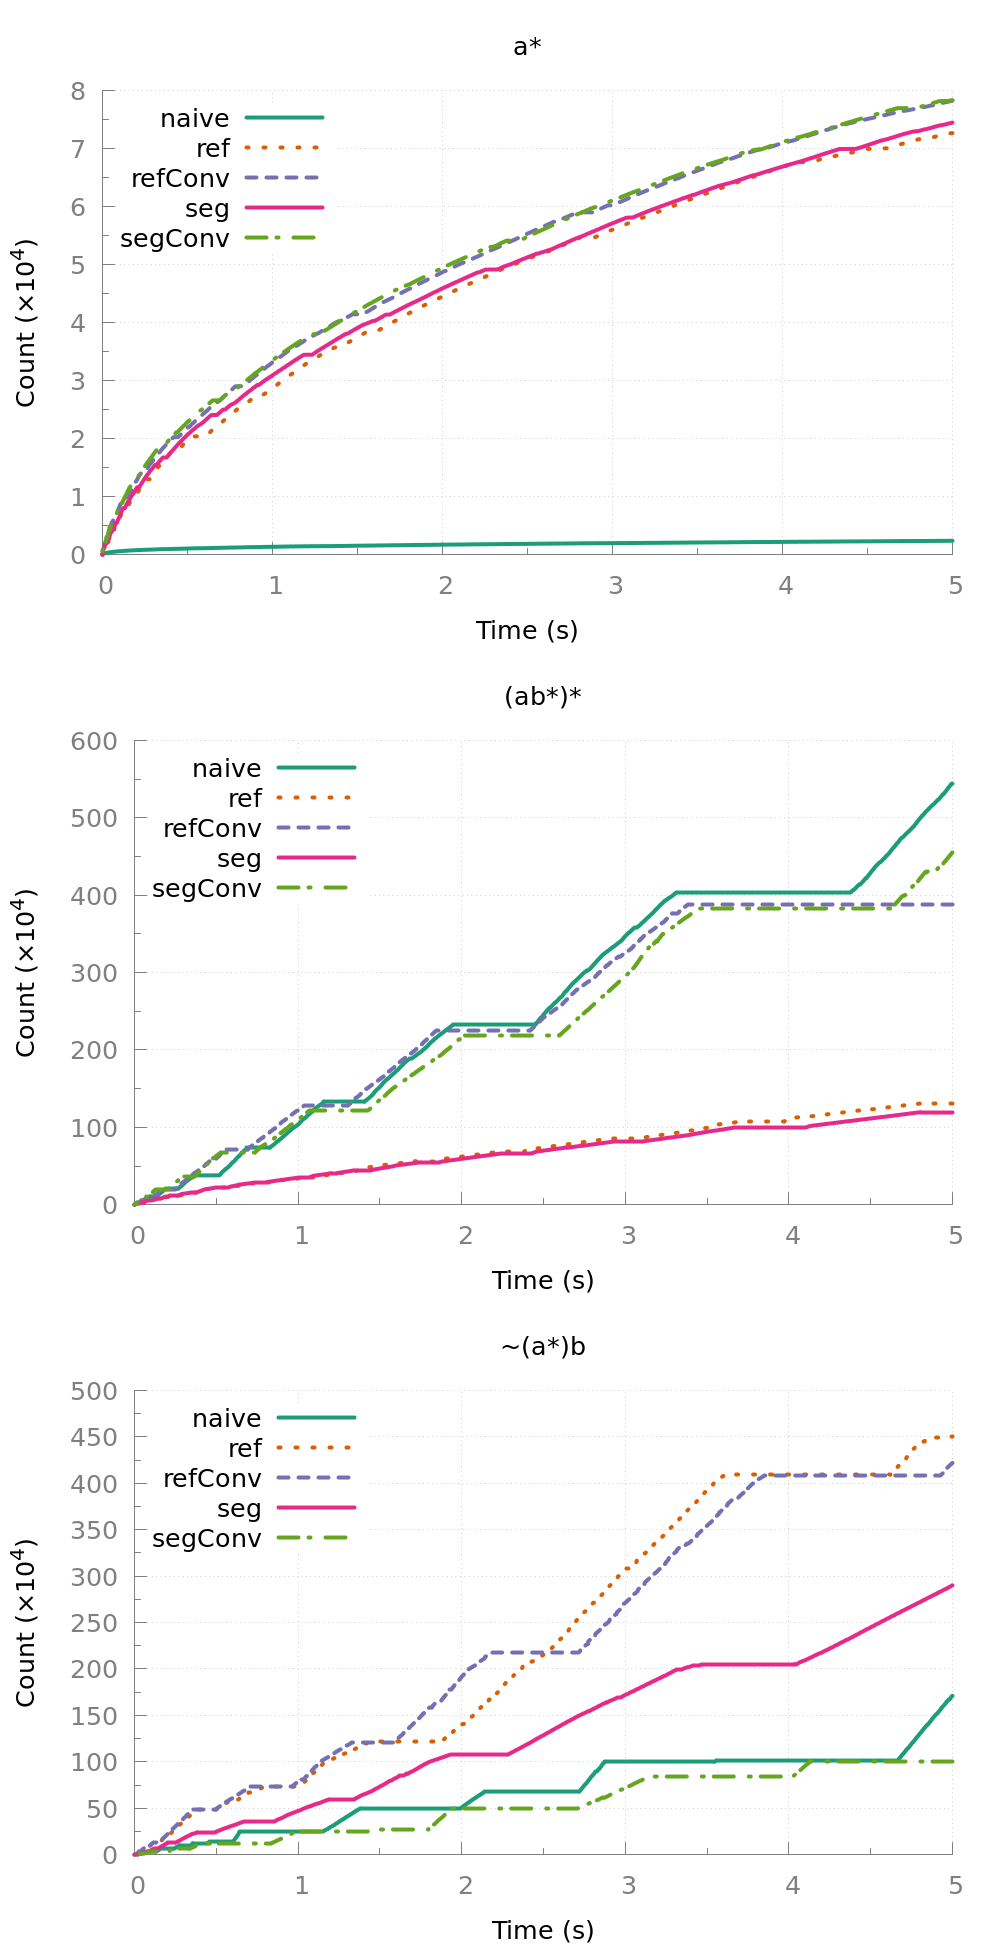
\includegraphics[width=\linewidth]{measure/haskell_all.png}
  \caption{Benchmark for the \haskell implementation with various algorithms}
  \label{bench:haskell:all}
\end{figure}
To evaluate the performance, we iterate through the stream of words
produced by the generator and force their evaluation.\footnote{In
  Haskell, forcing is done using \lstinline{Control.DeepSeq}.} Every
20 words, we record the time elapsed since the start of the iteration. We
stop the iteration after 5 seconds. The resulting graph plots the time (x-axis) against the number of words (y-axis) produced so far. The slope of the graph in indicates the generation speed of the plotted algorithm, high slope is correlated to high generation speed.  \cref{bench:haskell:all} contains the results for the Haskell implementations.

Most algorithms generate between 3000 and 150000 words in the first
second, which seems more than sufficient for testing purposes.
Regarding comparative performance, the \textbf{refConv} implementation
which uses symbolic segments and convolutions is consistently in the
leading group. Sometimes one of the other implementations is slightly
faster, but not consistently so. This observation validates that the
changes proposed in \cref{sec:improvements} actually lead to
improvements and suggests that \textbf{refConv} is the overall winner
of this comparison.

Looking at each graph in more detail, we can make the following
remarks:
\begin{itemize}[leftmargin=*]
\item All implementations are equally fast on $\Rstar a$ except
  the naive implementation, which  relies on list lookups without
  sparse indexing.
\item For $\Rstar{(\Rconcat{a}{\Rstar{b}})}$ and
  $\Rconcat{\Rcomplement{(\Rstar{a})}}{b}$, the graph of some implementations
  has the shape of ``skewed stairs''. We believe this phenomenon is due to
  insufficient laziness: when arriving at a new segment, part of the
  work is done eagerly which causes a plateau. When that part is done,
  the enumeration proceeds lazily.  As laziness and GHC
  optimizations are hard to control, we did not attempt to correct this.
\item $\Rstar{(\Rconcat{a}{\Rstar{b}})}$ demonstrates that sparse indexing
  does degrade performance when applying \code{star} to non-sparse languages.
  Using the convolution technique presented in \cref{sec:convolution} resolves this problem.
\item The \textbf{ref} and \textbf{refConv} algorithms are
  significantly faster on $\Rconcat{\Rcomplement{(\Rstar{a})}}{b}$
  compared to \textbf{seg} and \textbf{segConv}. We have no good
  explanation for this behavior as the code is identical up to the
  symbolic representation of full and empty segments. However, the
  only sublanguage where this representation could make a difference
  is $\Lang{b}$, which is also represented finitely by
  \textbf{segConv} and should thus benefit from the convolution
  improvement in the same way as \textbf{refConv}.
\end{itemize}


\subsection{Comparing Data Structures in the \ocaml Implementation}
\label{sec:bench:ocaml}
\begin{figure}[!tp]
  \centering
  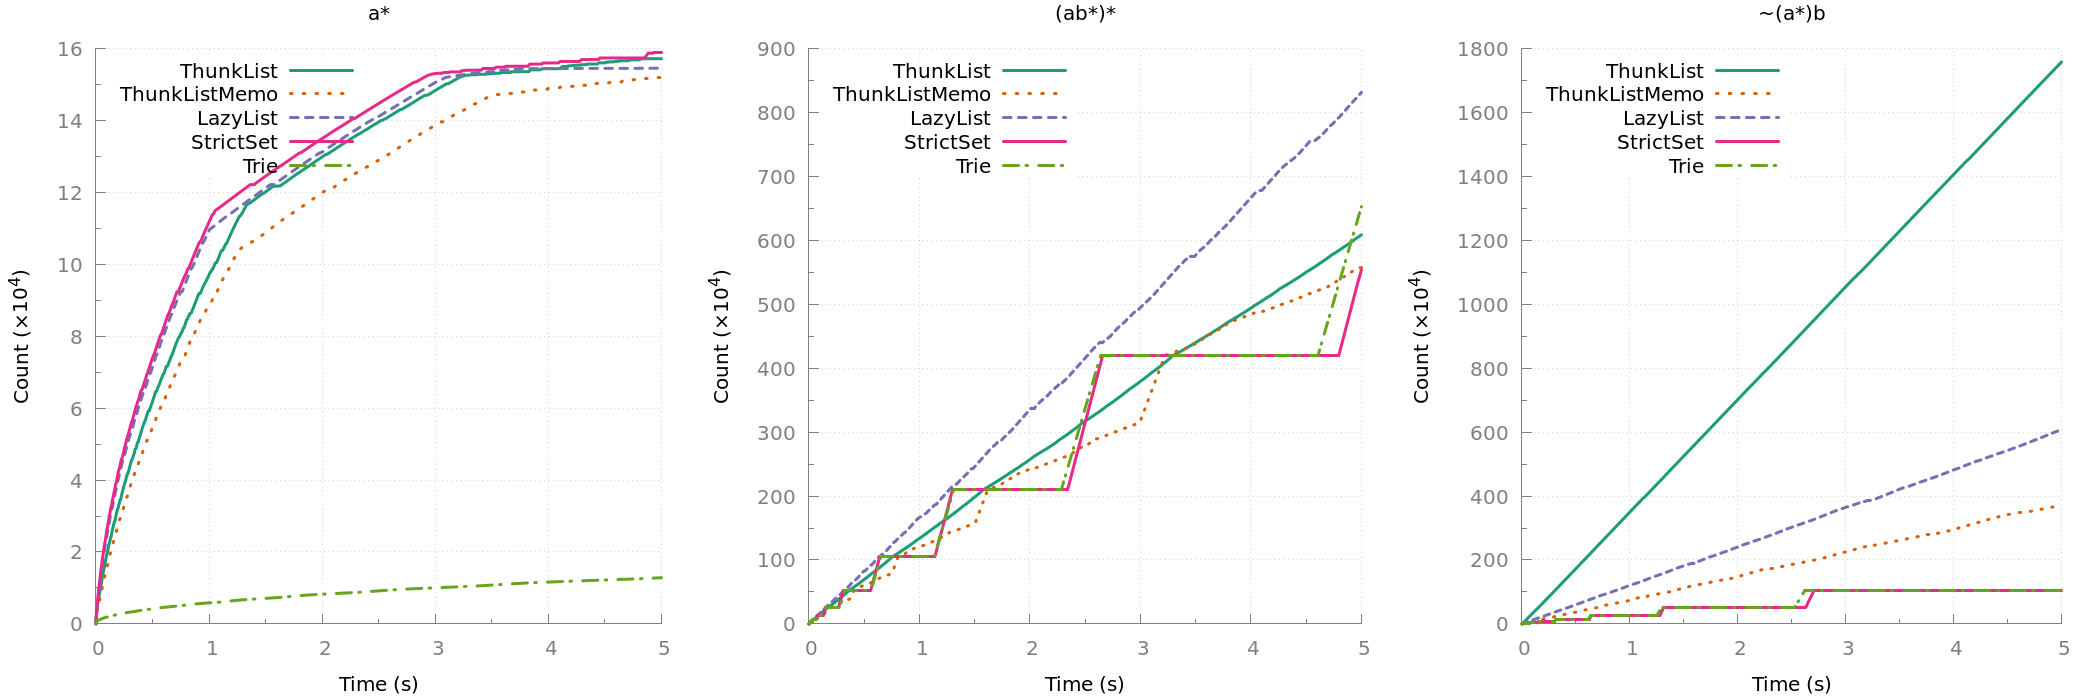
\includegraphics[width=\linewidth]{measure/ocaml_all.png}
  \caption{Benchmark for the \ocaml implementation with various data-structures}
  \label{bench:ocaml:all}
\end{figure}

By now, we have established that the \textbf{refConv} algorithm
provides the best overall performance.  The \haskell implementation,
however, essentially uses lazy lists to represent single language
segments. To measure the influence of strictness and the choice of data structure on
language generation, we consider the functorized \ocaml implementation, as it facilitates such experimentation.
We follow the same methodology as the \haskell evaluation using the
regular expressions $\Rstar a$, $\Rstar{(\Rconcat{a}{\Rstar{b}})}$ and
$\Rconcat{\Rcomplement{(\Rstar{a})}}{b}$.  The results are shown in
\cref{bench:ocaml:all}.

Unlike the previous benchmark for algorithms, there is no clear winner
among the data structures. The \code{ThunkList} and \code{LazyList} modules seem to
be superior to the alternatives, although the results are highly influenced by
the regular expression considered.
\begin{itemize}[leftmargin=*]
\item The \code{Trie} module is very inefficient on $\Rstar a$ because
  our implementation of tries does not use path compression.
  In the case of $\Rstar a$, where each segment contains only one word, the
  trie degenerates to a list of characters.
  We believe
  an implementation of tries with path compressions would perform significantly better.
\item The other data structures exhibit a very pronounced slowdown on $\Rstar a$
  when reaching 150000 words.
  We believe this slowdown is due to garbage collection because
  the active heap contained 10G of data before
  a collection was triggered. Much less memory is consumed for the other regular
  expression.
\item The strict data structures showcase a very marked ``skewed
  stair'' pattern, which is completely absent for \code{ThunkList} and
  \code{LazyList}. Thus, manual control of laziness works very well in
  \ocaml. These results also demonstrate that strict data structures
  should only be used when all elements up to a given length are
  needed. In such a case the stair pattern causes no problems.
\item Memoization for thunk lists significantly degrades performance. It seems
  that the linear cost of memoizing the thunk list and allocating the vectors
  is higher than simply recomputing lists.
\end{itemize}


\begin{figure}[!tp]
  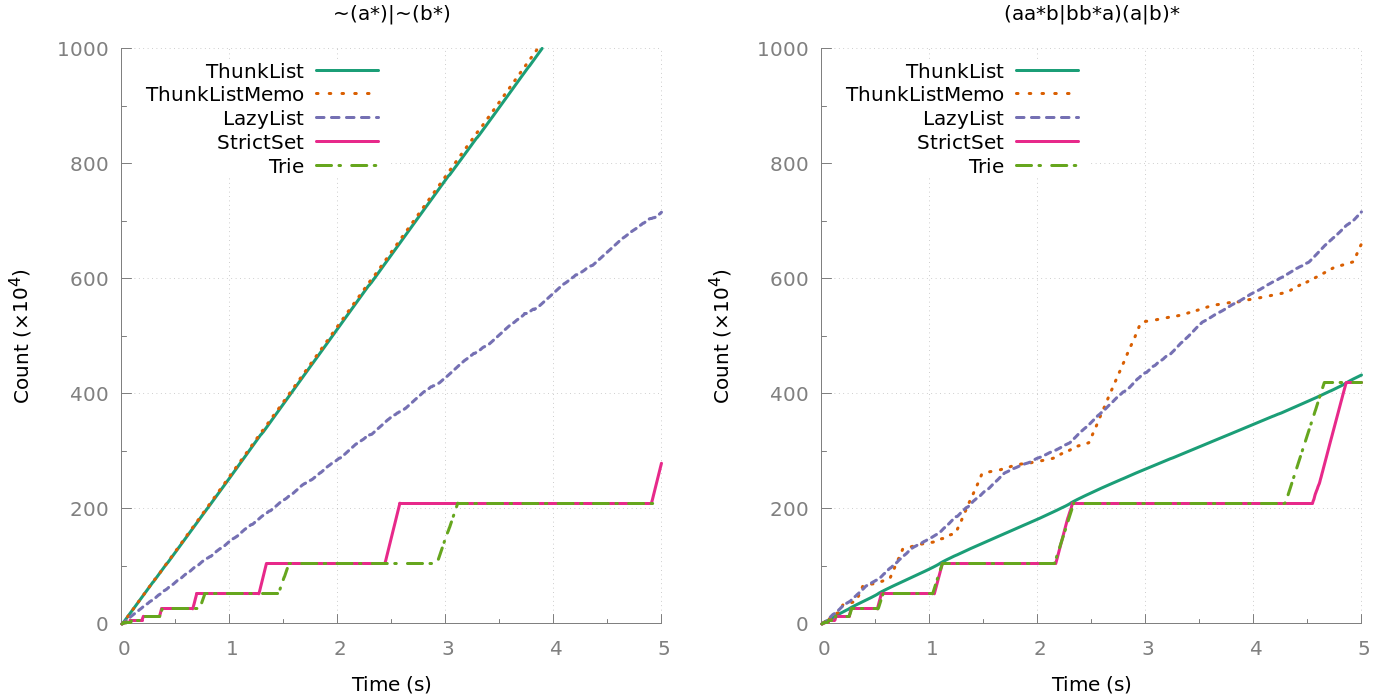
\includegraphics[width=\linewidth]{measure/ocaml_union.png}
  \caption{Benchmarking \texttt{union} in the \ocaml data-structures}
  \label{bench:ocaml:union}
\end{figure}

While the regular expressions presented previously do exercise
\code{concatenation} and \code{star}, they do not exercise set
operations.  To test set operations on non-trivial segments (that are
neither full nor empty), we consider the language of words with at
least one $a$ and one $b$. This language can be built in two ways:
$\Rintersect{\Rcomplement{(\Rstar{a})}}{\Rcomplement{(\Rstar{b})}}$
and $\Rconcat{(\Runion{a\Rstar{a}b}{b\Rstar{b}a})}{\Rstar{\Sigma}}$.
The first expression applies {intersection} to two large languages,
the second expression takes the union of smaller languages, but uses a
concatenation.  The performance of the various data structures on
these two regular expressions are presented in
\cref{bench:ocaml:union}.  Lazy and thunk lists, with or without
memoization, are very efficient on the union and intersection of
languages but less so when concatenation is involved. Performance of
strict sets and tries is surprisingly poor.

\subsection{The Influence of Regular Expressions on Performance}
\begin{figure*}[tp]
  \centering
  \begin{subfigure}[t]{0.5\linewidth}
    \centering
    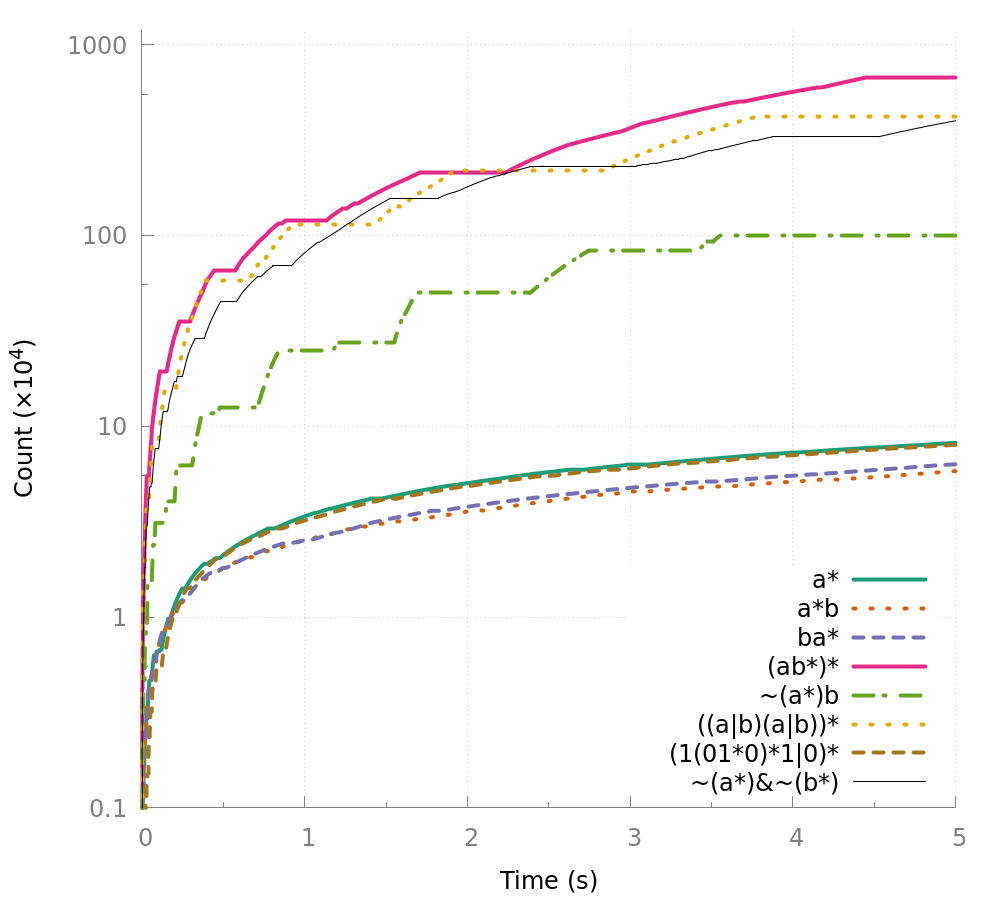
\includegraphics[width=\linewidth]{measure/haskell_langs.png}
    \caption{\haskell implementation with \code{segConv}}
    \label{bench:haskell:langs}
  \end{subfigure}~
  \begin{subfigure}[t]{0.5\linewidth}
    \centering
    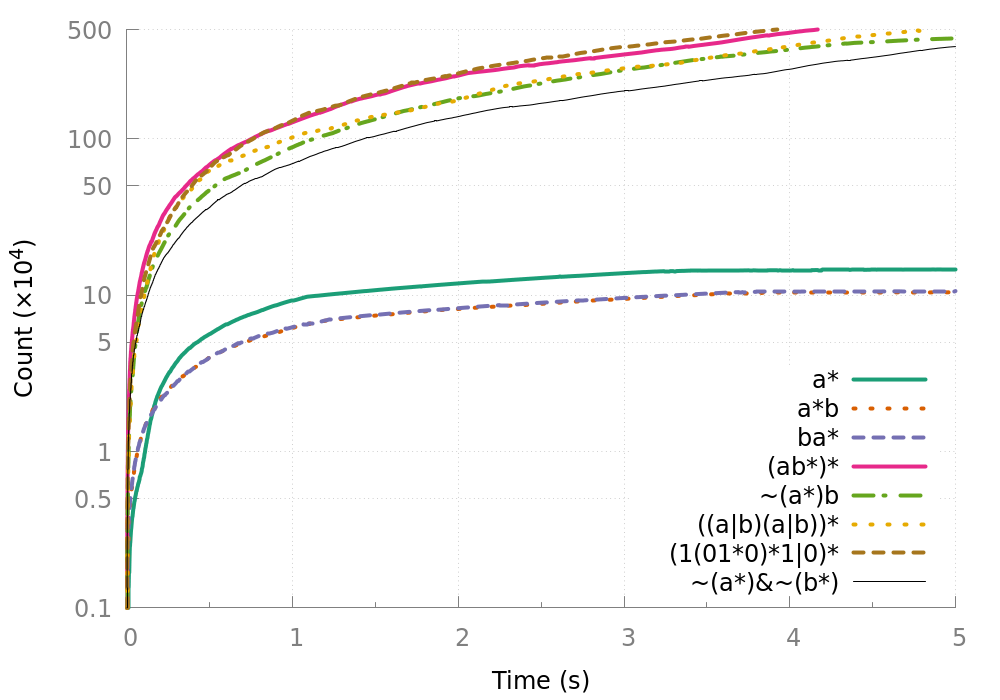
\includegraphics[width=\linewidth]{measure/ocaml_langs.png}
    \caption{\ocaml implementation with \code{ThunkList}}
    \label{bench:ocaml:langs}
  \end{subfigure}
  \caption{Benchmark on different regular expressions}
  \label{bench:langs}
\end{figure*}

The benchmark results so far demonstrate that the performance of the language
generator highly depends on the structure of both
the generated language and the regular expression considered.
To further explore this observation we compare a range of regular expressions
with the \code{refConv} \haskell implementation and the \code{ThunkList}
\ocaml implementation.
Before presenting the results, a word of warning:
We do not claim to offer a fair comparison between languages!
The two implementations are not exactly the same and we made no attempt
to measure both language under exactly the same conditions.

\cref{bench:langs} contains the resulting graphs.  These graphs use a
logarithmic scale for the word count as it enables better comparison
between the regular expression specimens.

We add three new regular expressions to the range of expressions already considered:
\begin{itemize}
\item $\Rstar{(\Sigma\Sigma)}$, the language of words of even
  length. This language is neither finite nor cofinite, but it can make
  good use of the symbolic representation of segments.\footnote{This
    language has $P (w \in L) = 0.5$ thus solving the exercise posed
    earlier.}
\item $\Rstar{(\Runion{1 \Rstar{(0\Rstar{1}0)}1}{0})}$, the language
  of multiples of 3 written in binary representation. Again, this is a language that is neither
  finite nor cofinite, but its segments are never full nor empty.
\item $\Rstar{a}b$ and $b\Rstar{a}$, which together check whether
  {concatenation} behaves symmetric with respect to performance.
\end{itemize}

Languages are roughly ordered by size/density, i.e., $P (w\in L)$. We
observed that the bigger the segments of a language, the faster it is
to generate its words.  If each segment contains many words, we do not
need to compute many segments to generate a large number of words.
Moreover, most operations, notably those involving the product of
segments, are more expensive when considering segments of higher
indices. Briefly put, long strings are harder to generate than short
ones.

Regarding symmetry, we find that the generation of $\Rstar{a}b$ and
$b\Rstar{a}$ has the same performance in both implementations,
thanks to the improved convolution technique
with detection of finite languages described in \cref{sec:convolution}.



%%% Local Variables:
%%% mode: latex
%%% TeX-master: "main"
%%% End:
